
\chapter{ארכיטקטורת \textenglish{BiLSTM} לחילוץ אותות}

\section{רשתות \textenglish{LSTM} ומבנה השערים}

רשת \textenglish{LSTM} \cite{hochreiter1997lstm} מרחיבה את ה-\textenglish{RNN} הקלאסית על ידי הוספת שלושה שערים: שער שכחה (\textenglish{forget gate}), שער כניסה (\textenglish{input gate}) ושער יציאה (\textenglish{output gate}). הגדרות השערים:

\begin{equation}
f_t = \sigma(W_f [h_{t-1}, x_t] + b_f), \quad
i_t = \sigma(W_i [h_{t-1}, x_t] + b_i)
\end{equation}

\begin{equation}
c_t = f_t \odot c_{t-1} + i_t \odot \tanh(W_c [h_{t-1}, x_t] + b_c)
\end{equation}

מבנה זה מאפשר לרשת לשמור מידע לאורך רצפים ארוכים ולהתמודד עם בעיית ה-\textenglish{vanishing gradient} שפוגעת ב-\textenglish{RNN} רגילות.

\section{ארכיטקטורת \textenglish{Encoder-Decoder} דו-כיווני}

הארכיטקטורה שלנו מורכבת משני חלקים: מקודד \textenglish{BiLSTM} (\textenglish{Bidirectional LSTM}) המעבד את הרצף בשני כיוונים, ופוענח המשחזר את הפרמטרים הסינוסואידליים. ה-\textenglish{BiLSTM} מאפשר לכל נקודת זמן גישה להקשר עתידי ועבר, יתרון קריטי בזיהוי פרמטרים תדרים.

\section{שילוב עם מנגנון קשב}

שילוב \textenglish{cross-attention} בין המקודד לפוענח \cite{vaswani2017attention} מאפשר לפוענח להתמקד בחלקים הרלוונטיים ביותר של הספקטרוגרמה בכל צעד חיזוי. זה משפר את הדיוק בחילוץ מרכיבים תדריים סמוכים (\textenglish{close frequencies}) שללא קשב עשויים להתבלבל ביניהם.

\begin{figure}[H]
\centering
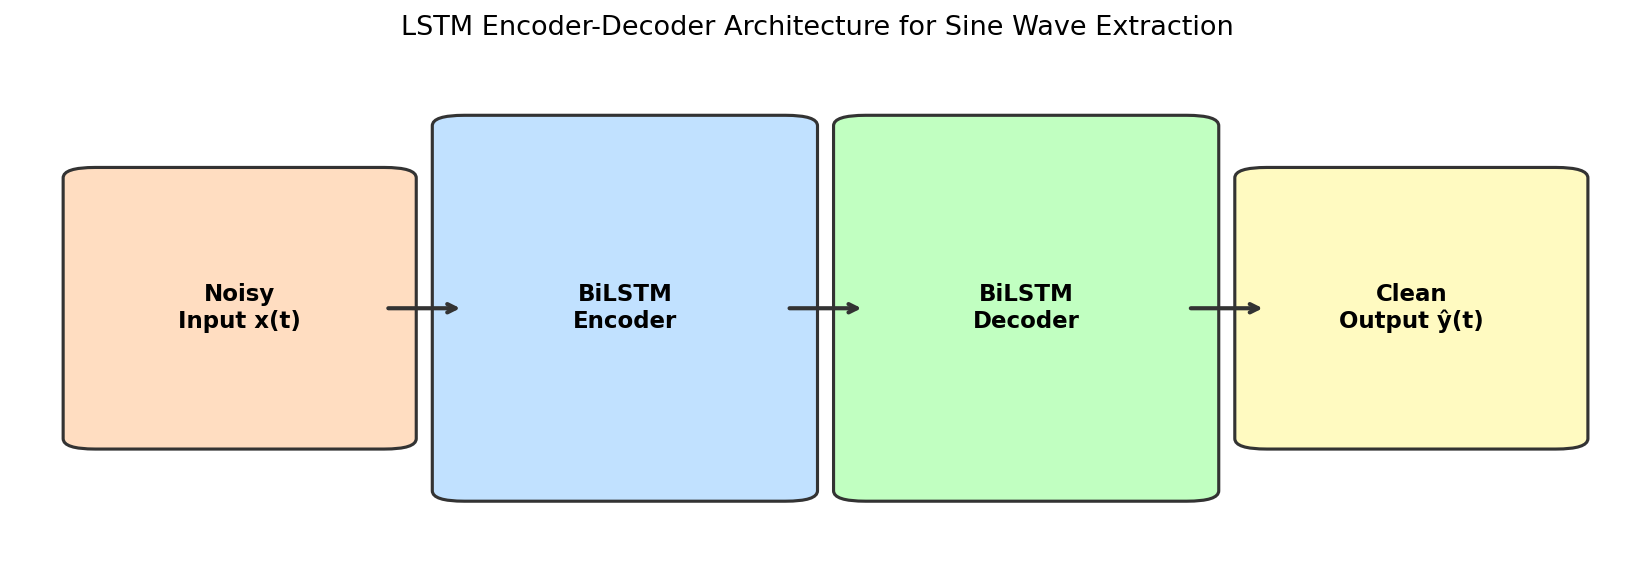
\includegraphics[width=0.82\textwidth]{assets/architecture.png}
\caption{\textenglish{BiLSTM Encoder-Decoder Architecture for Signal Extraction}}
\label{fig:arch}
\end{figure}
